\chapter[Visualization on the Web]{Visualization\\ on the Web}
\label{chap:visualization_web}

% Position the image to the right of the heading.
\vspace{-9\baselineskip} % move up
\hfill
 \begin{minipage}{0.5\textwidth}
 \centering
 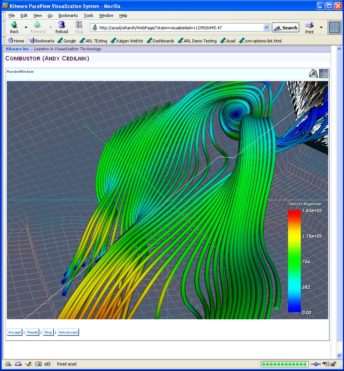
\includegraphics{VTKTextbook-269}
  \captionof*{figure}{\textit{Streamline visualization with ParaView Enterprise Edition.}}
 \end{minipage}
\vspace{2\baselineskip}

\firstletter{T}he early 1990s established the widespread use and accessibility of the World Wide Web.
Once a network used primarily by researchers and universities, the Web has become something that is used by people throughout the world.
The effects of this transformation have been significant, ranging from personal home pages with static images and text, to professional Web pages embedding animation and virtual reality.
This chapter discusses some of those changes and describes how the World Wide Web\index{World Wide Web} can be used to make visualization more accessible, interactive, and powerful.
Topics covered include the advantages and disadvantages of client-side versus server-side visualization, VRML, and Java3D, interwoven with demonstration examples.

\section{Motivation}
Before describing in detail how to perform visualization over the Web, it is important to understand what we expect to gain. Clearly people have been visualizing data prior to the invention of the Web, but what the Web adds is the ability for people throughout the world to share information quickly and efficiently.
Like all successful communication systems, the Web enables people to interact and share information more efficiently compared to other methods.
In many ways the Web shares the characteristic of computer visualization in its ability to communicate large amounts of data.
For that reason, computer graphics and visualization are now vital parts of the Web, and are becoming widespread in their application.

To demonstrate these concepts we provide a simple example that illustrates the usefulness of the Web, and leads us into our first important topic: client--side versus server--side visualization.

One common problem for researchers has been how to share or publish results. Typically, this involved having one site perform the research, interact with the data, form conclusions, and then publish the results as a report. The report might include a few pictures and possibly even a short animation. Obtaining access to the report might be through a journal or conference. Subsequently, co--workers at other sites would read the report and respond via verbal communication or formal articles.

While certainly a viable means of sharing information, there are two important shortcomings in such a scenario. First, the report does not allow another researcher to interact with the visualizations. They are static pictures or pre--recorded animations. There is no opportunity to look from a different angle or change the parameters of the visualization. Second, access to the report may be limited or untimely. For example, some journals require as much as two years to accept, review, and publish an article. This time delay is too long for many technology-driven fields such as medicine, computers, or business. Such delays in receiving information can result in fruitless research or a failed business.

Using the Web this scenario changes significantly. It is now possible to create reports so that other researchers can interact directly with the data, including visualizing the results in an alternative form. The Web also provides the opportunity to publish results immediately so that anyone with Web access can view them. Additionally, results can be modified as your work progresses so that they are always up to date.

Another motivation for visualization over the Web is collaboration. If a researcher is performing a visualization of a dataset at one site, there are a number of hurdles preventing someone at another site from doing the same. For starters, the data, which could be sizable, must be copied, or sent from one site to the other. Then the software being used must be available at both sites which may not even be possible depending on the hardware available. The popularity of cross--platform systems such as AVS, IBM's Data Explorer, and VTK have helped this situation, but even then the software and data reside at both locations. This is frequently referred to as client-side visualization because all steps of the visualization are performed at the collaboration (or client) sites. In contrast, server-side visualization occurs when all of the visualization is done at one centralized location called the server. The results of the server-side visualization are then sent to collaboration sites.

The Web opens up the opportunity to perform mixed client/server visualization that has a number of benefits. First, let's consider the drawbacks to client-side only visualization. As mentioned in the preceding discussion, client--side visualization requires both the data and the software at the client. If the datasets are very large it may be impractical to transfer the data over the Web. Since the server doesn’t know what the client is going to do with the data, all of the data must be sent. Additionally, the client may not have sufficient memory or performance to perform the visualization. The advantages of client-side visualization are that the user has complete control over the visualization and can interact with or modify it at will.

With server-side visualization the most significant loss is in interaction. A server--side only visualization is much like publishing a report. The clients have very little control over the images and animations it produces. The advantage is that the results are easily viewed from any client without requiring special hardware or software. As we will see in the remaining sections, the advantage of using recently developed Web technology is that we can mix server--, and client--side visualization much more readily than before, providing the benefits of both.

\section{Early Web Visualization}

While the World Wide Web received most of its attention in the early 1990s, its foundations date back decades earlier to the Internet and ARPAnet. What made the 1990s so significant was the development of some standardized visual tools for exchanging information. The most common of these are the Web browsers such as Mosaic, Netscape Navigator, and Microsoft Internet Explorer. These browsers provide a unified interface supporting many data (or content) types. The first content type to gain wide acceptance was HyperText Markup Language or HTML. HTML provides a way to format text and images in a document that can be shared across the Web. HTML also includes the ability to provide active links in one document that point to other documents on the Web. This helps to solve the problem of sharing results but it still limits the user to static images.

This problem was quickly solved as Web browsers started to support other content types including animation formats such as MPEG, AVI, and QuickTime. Now a link in a HTML document can load an animation sequence for the user to view and interact with. The next step was to allow the client to control the generation of the animation sequence on the server. To facilitate this process, a mechanism for the client to send general information to the server was introduced. The Common Gateway Interface (CGI) along with HTML forms serves this purpose. In this two-pronged approach, an HTML form collects information from the client, passes it to the server that executes a CGI-BIN script, and then finally produces a result for the client to view.

\begin{figure}[htb]
    \centering
	\begin{subfigure}[h]{0.76\linewidth}
		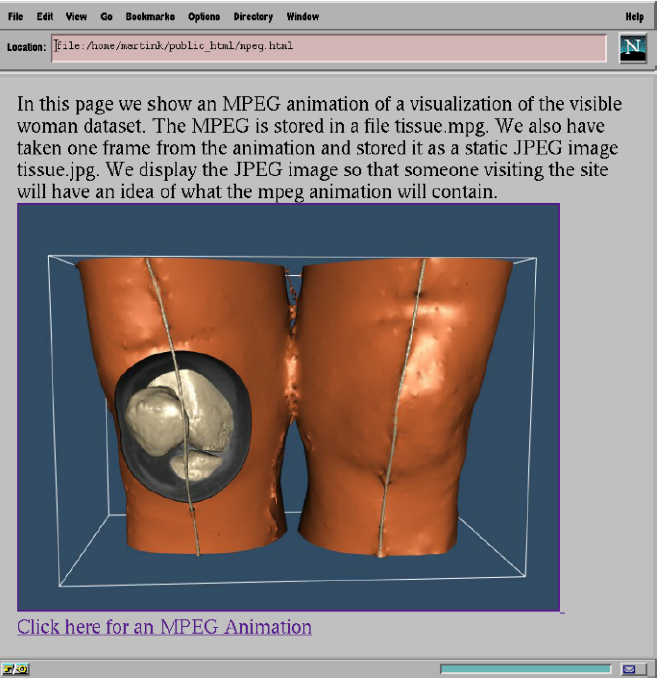
\includegraphics[width=0.96\linewidth]{Figure11-1a}
		\captionsetup{justification=centering}
		\caption*{}
		\label{fig:Figure11-1a}
	\end{subfigure}
	\hfill
	\begin{subfigure}[h]{0.98\linewidth}
       \begin{lstlisting}[language=HTML,  caption={}, numbers=none, frame=none]
        <HEAD><TITLE>Sample MPEG Animation Page</TITLE></HEAD>
        In this page we show an MPEG animation of a visualization
        of the visible woman dataset. The MPEG is stored in a file
        tissue.mpg. We also have taken one frame from the animation
        and stored it as a static JPEG image tissue.jpg. We display
        the JPEG image so that someone visiting the site will
        have an idea of what the mpeg animation will contain.
        
        <br>
        <A HREF="tissue.mpg"><IMG SRC="tissue.jpg">
        <br>Click here for an MPEG Animation</A>
        \end{lstlisting}
        \label{fig:Figure11-1b}
	\end{subfigure}
	\caption{MPEG visualization example.}\label{fig:Figure11-1}
\end{figure}

For example, consider a situation where you would like to perform an isosurface extraction from volume data and then generate a short animation rotating the camera around the isosurface. There are a number of ways to generate such an animation and create an MPEG file, which can then be linked into an HTML document. Figure \ref{fig:Figure11-1} shows one example generated and the associated HTML code.

\begin{figure}[htb]
    \centering
	\begin{subfigure}[h]{0.76\linewidth}
		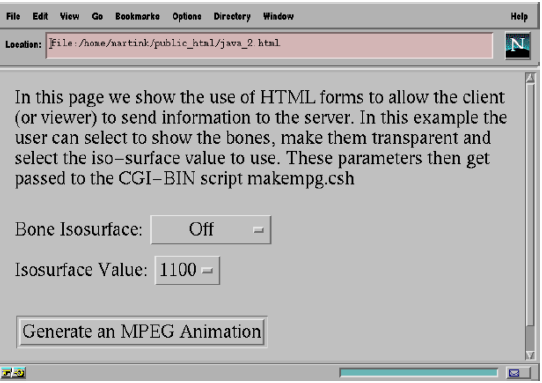
\includegraphics[width=0.96\linewidth]{Figure11-2a}
		\captionsetup{justification=centering}
		\caption*{}
		\label{fig:Figure11-2a}
	\end{subfigure}
	\hfill
	\begin{subfigure}[h]{0.98\linewidth}
       \begin{lstlisting}[language=HTML,  caption={}, numbers=none, frame=none]
        <HEAD><TITLE>Sample MPEG Animation Page</TITLE></HEAD>

        <FORM METHOD="POST" ACTION="/cgi-bin/makempg.csh">

        In this page we show the use of HTML forms to allow the client
        (or viewer) to send information to the server. In this example
        the user can select to show the bones, make them transparent and
        select the isosurface value to use. These parameters then get
        passed to the CGI-BIN script makempg.csh</P>

        <P>Bone Isosurface: <SELECT NAME=iso>
        <OPTION SELECTED>Off

        <OPTION>On
        <OPTION>Transparent
        </SELECT><BR>
        Isosurface Value: <SELECT NAME=isoval>
        <OPTION>1400 <OPTION>1200
        <OPTION SELECTED>1100
        <OPTION>1000 <OPTION>900
        </SELECT><BR>

        <P><INPUT TYPE="submit"
        VALUE="Generate an MPEG Animation"></FORM></P>
        \end{lstlisting}
        \label{fig:Figure11-2b}
	\end{subfigure}
	\caption{Example HTML form.}\label{fig:Figure11-2}
\end{figure}

he title and text description are followed by \texttt{<A HREF=''tissue.mpg''>} which associates the MPEG file, \texttt{tissue.mpg}, with whatever comes between the first \texttt{<A>} and the closing \texttt{</A>}. In this example there is a JPEG image and a line of text. Clicking on either of these will play the MPEG animation.
Now let's use CGI and an HTML form to enable the client to change the isosurface value. The first step is to obtain the desired isosurface value from the client using an HTML form such as Figure \ref{fig:Figure11-2}. The HTML code is also shown.

The FORM keyword starts the definition of the HTML form. The \texttt{ACTION} keyword indicates what should happen when the form is submitted. In this example the server will run a \texttt{CGI-BIN} script called \texttt{makempg.csh} when a client submits this form. Next the two pull-down menus are declared with the \texttt{SELECT} keyword. The `NAME` keyword sets up an association between a string name and the value for this menu. This will be used by the script \texttt{makempg.csh} to access the values from the form. The \texttt{OPTION} and \texttt{SELECTED} keywords provide a mechanism to specify the values for the menu and what value the default should be. Finally, the last two lines create the button that will submit the form when pressed.

Once the client has submitted the form, the server will execute the `CGI-BIN` script and pass it the arguments from the form. The script will then generate a new MPEG animation based on the client's request and return it to the client.

While these examples demonstrate a closed loop of interaction between the client and server, there are two remaining problems. First, this approach places the entire computational load on the server. While this may be viable for some applications, some servers literally receive millions of client requests a day, severely straining server resources. Second, while the process is interactive, the lag time between making a change and seeing the result can be considerable, depending on the length of the animation and the communication bandwidth. Better solutions are now available to improve interactivity.

\section{Virtual Reality Modeling Language (VRML)}

HTML is a powerful tool for creating hypertext documents; however, it does not directly support 3D content. This limitation can be severe if we are interested in exploring 3D data, and do not know exactly what we wish to see, or what we wish to present to a user. As a result, an important development has been to create 3D worlds that the user can freely navigate. One application of this technology is Web content that allows customers to preview a hotel, resort, or vacation area by moving through a model representing the site. Such an application allows customers to preview a prospective business and directly experience what is available without relying on preconstructed views of the site.

As a result of this need for greater interactivity, a new content type appeared referred to as the Virtual Reality Modeling Language (VRML). The idea behind VRML was to create a standard definition for transmitting 3D content over the Web. Having its origins in an early system called Labyrinth, which is in turn based on Reality Lab from Rendermorphics, it quickly evolved to the VRML 1.0 specification based on Open Inventor from Silicon Graphics.

\begin{figure}[!htb]
	\centering
	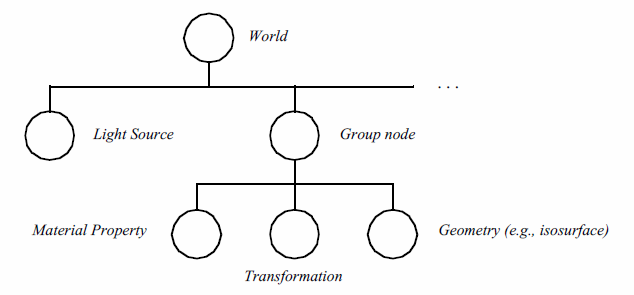
\includegraphics[width=0.84\textwidth]{Figure11-3}
	\caption{A simple scene graph.}
	\label{fig:Figure11-3}
\end{figure}

A VRML 1.0 file (typically with a .wrl extension, abbreviated from world) contains a scene graph representation of a 3D world (e.g., a scene). Consider Figure \ref{fig:Figure11-3} which shows a simple scene. It is a directed graph that is traversed depth first from top to bottom with the content of the graph in its nodes (the circles). In this figure the top node is a group node that collects child nodes together. The light is a directional light node and the second group node represents an isosurface. The isosurface group node is represented by three children nodes: one to control the material properties, a general transformation, and finally the 3D geometry. VRML and Open Inventor\index{OpenInventor} support Geometry (e.g., isosurface) many different types of nodes including some support for animation. (See also ``Alternative Visual Programming Models''  on page \pageref{subsec:alternative_visual_programming_models} for more information).

The basic idea behind VRML 1.0 is that the 3D content can be downloaded from the server and then interacted with the client. There are many Web browsers that support VRML and most take advantage of client-side graphics hardware if available. This helps address both the server-load problem and the interaction lag time associated with the earlier approach of server-generated MPEG animations. Like HTML, VRML supports active links so that navigating through a door in one VRML world can send you to new VRML (or HTML) sites.

To address many of the limitations in VRML 1.0, significant changes were made resulting in the VRML 2.0 standard. Where VRML 1.0 was primarily a static scene description with some very limited behaviors, VRML 2.0 adds audio, video, and integration with Web scripting languages and more. It is still essentially a data file, but with the capabilities of simulating much more realistic and immersive environments. Many visualization systems, including VTK, support exporting scenes as VRML files. Consider the following example:

\begin{lstlisting}[language=TCL, caption={}, numbers=none, frame=none, escapechar=\%]
%\index{vtkPLOT3DReader!VRML example}%
vtkRenderer ren1
vtkRenderWindow renWin
  renWin AddRenderer ren1

# create pipeline
#
vtkPLOT3DReader%\index{vtkPLOT3DReader!example}% pl3d
  pl3d SetXYZFileName "$VTK_DATA_ROOT/Data/combxyz.bin"
  pl3d SetQFileName "$VTK_DATA_ROOT/Data/combq.bin"
  pl3d SetScalarFunctionNumber 100
  pl3d SetVectorFunctionNumber 202
vtkContourFilter%\index{vtkContourFilter!example}\index{vtkContourFilter!VRML example}% iso
  iso SetInputConnection [pl3d GetOutputPort]
  iso SetValue 0 .38
vtkPolyDataNormals%\index{vtkPolyDataNormals!example}\index{vtkPolyDataNormals!VRML example}% normals
  normals SetInputConnection [iso GetOutputPort]
  normals SetFeatureAngle 45
vtkPolyDataMapper%\index{vtkPolyDataMapper!example}\index{vtkPolyDataMapper!VRML example}% isoMapper
  isoMapper SetInputConnection [normals GetOutputPort]
   isoMapper ScalarVisibilityOff
vtkActor%\index{vtkActor!VRML example}% isoActor
  isoActor SetMapper isoMapper
  eval [isoActor GetProperty] SetColor 0.3 0.4 0.5

vtkStructuredGridOutlineFilter%\index{vtkStructuredGridOutlineFilter!example}% outline
  outline SetInputConnection [pl3d GetOutputPort]
vtkPolyDataMapper outlineMapper
  outlineMapper SetInputConnection [outline GetOutputPort]
vtkActor outlineActor
  outlineActor SetMapper outlineMapper

# Add the actors to the renderer, set the background and size #
ren1 AddActor outlineActor ren1 AddActor isoActor
renWin SetSize 500 500
ren1 SetBackground 0.1 0.2 0.4
\end{lstlisting}

This is a typical program within VTK that extracts an isosurface and bounding outline from a structured grid dataset. To export this result to a VRML data file we can use the vtkVRMLExporter\index{vtkVRMLExporter} as shown below:

\begin{lstlisting}[language=TCL, caption={}, numbers=none, frame=none]
vtkVRMLExporter exp
  exp SetRenderWindow renWin
  exp SetFileName Combustor.wrl
  exp Write
\end{lstlisting}

These four lines create an instance of vtkVRMLExporter\index{exporter!VRML}\index{vtkVRMLExporter!example}, set its input to renWin (an instance of vtkRenderWindow), set a file name, and finally write out the result. This is different from previous examples where data was written out using vtkPolyDataWriter or other subclasses of vtkWriter. vtkVRMLExporter is a subclass of vtkExporter\index{vtkExporter}, not vtkWriter. The significant difference is that a writer takes a vtkDataSet as input and is responsible for writing out a single dataset. An exporter takes a vtkRenderWindow as input and is responsible for writing out an entire scene, possibly containing multiple actors, lights, textures, and material properties, in addition to any datasets.

If you consider a continuum from a static data file to a fully interactive visualization program, vtkWriter would be at one end, vtkExporter in the middle, and a VTK program at the other. VRML 1.0 would fall at the same place as vtkExporter and VRML 2.0 would fall between vtkExporter and an actual program due to its added support for behavior and script interaction. What VRML lacks from a visualization perspective is algorithms. VRML is a 3D multimedia content format and lacks direct support for applying visualization techniques or algorithms.

\section{A VRML Visualization Server}
\index{server!VRML|(}\index{VRML!visualization server|(}\index{visualization!using VRML|(}\index{VRML!example|(}

We can improve on the earlier MPEG visualization server example by creating a VRML visualization server. The primary limitations of the MPEG approach were that the processing burden was on the server, and the client-side interaction was limited to requesting that a different MPEG animation be generated. In our improved example, the basic idea is the same as before. That is, we use a HTML form to define parameters for a visualization, which then spawns off a CGI-BIN script. The difference is that in this example the server will generate a VRML data file that is returned to the client. The client can then control the viewpoint and rendering of the VRML result. The data and visualization software still reside on the server, so the client is only required to have a VRML compatible Web browser.

The HTML form is essentially the same as the one used to generate Figure \ref{fig:Figure11-2}. What changes is that the \texttt{CGI-BIN} script now needs to produce a \texttt{VRML} file instead of an \texttt{MPEG}. So instead of the form invoking \texttt{makempg.csh}, it will invoke a C++ executable named \texttt{VRMLServer}. This executable will parse the inputs from the form and then write out a \texttt{VRM}L file to its standard output. The first part of the program parses the arguments from the form. The server passes these arguments as a single string to the program's standard input. At the same time an environment variable named \texttt{CONTENT\_LENGTH} is set to the length of this input. In this example there are two values passed from the form: iso and isoval. According to convention they are separated by a ``\&'' when passed to the \texttt{CGI-BIN} script. The following C++ code extracts these values from the input string and performs some quick error checking.

\begin{lstlisting}[language=C++, caption={}, numbers=none, frame=none]
// first get the form data
env = getenv("CONTENT_LENGTH");
if (!env) return -1;
int inputLength = atoi(env);
// a quick sanity check on the input
if ((inputLength > 40)||(inputLength < 17)) return -1;
cin >> arg1;

if (strncmp(arg1,"isoval=",7) == 0)
  {
  isoval = atof(arg1 + 7);
  strcpy(isoType,arg1 + 11);
  }
else
  {
  isoval = atof(arg1 + inputLength - 4);
  strncpy(isoType,arg1 + 4,inputLength - 16);
  isoType[inputLength - 16] = ‘\0’;
  }
\end{lstlisting}

This code is specific to the parameters in this example, but generic argument extraction routines such as cgic (see \href{https://boutell.com/cgic/}{cgic}) can be used. Once the form data has been obtained, it can be used to set up the visualization pipeline as usual. In the following code, an isosurface is added to the renderer based on the isoType input from the form. Likewise if isoType is set to ``Transparent'' then that actor's opacity is set to 0.5.

\begin{lstlisting}[language=C++, caption={}, numbers=none, frame=none]
// should we do the isosurface
if (strcmp(isoType,"Off"))
  {
  ren1->AddActor( isoActor );
  }
if (strcmp(isoType,"Transparent") == 0)
  {
  isoActor->GetProperty()->SetOpacity( 0.5 );
  }
\end{lstlisting}

Once the pipeline is set up, the last step is to generate the proper headers and VRML output. The header is the keyword Content-type: followed by the keyword x--world/x--vrml that is the specification for VRML content. This is often followed by a pragma indicating that the client browser should not cache the data, typically because of the memory it would consume.

\begin{lstlisting}[language=C++, caption={}, numbers=none, frame=none]
// Send out vrml header stuff
fprintf(stdout,"Content-type: x-world/x-vrml\n");
 fprintf(stdout,"Pragma: no-cache\n\n");
// write out VRML 2.0 file
vtkVRMLExporter *writer = vtkVRMLExporter::New();
  writer->SetInput( renWin );
  writer->SetFilePointer( stdout );
  writer->Write();
\end{lstlisting}

Finally an instance of vtkVRMLExporter\index{export!VRML}\index{vtkVRMLExporter!example} is created, assigned an instance of vtkRenderWindow as input, and set to write to standard output. When the Write() method is applied, the exporter updates the visualization pipeline and produces the VRML output. The vtkRenderWindow is never rendered and no windows appear on the server. There is no need for an interactor because the interaction will be handled by the client's VRML browser. This program simply reads in a string of input (the parameters from the form) and then produces a string of output (the VRML data). It is also important to remember that CGI--BIN scripts are typically run from a different user id and environment than your own; file names and paths should be fully specified.
\index{server!VRML|)}\index{VRML!visualization server|)}\index{visualization!using VRML|)}\index{VRML!example|)}

\section{Visualization with Java}
\index{Java|(}\index{visualization!using Java|(}\index{VTK!and Java|(}

The examples discussed so far have addressed Web-based visualization in a number of ways. We have seen how to present preconstructed content such as images and animations using HTML, as well as creating interactive worlds with VRML. Each technique has its benefits but lacks the flexibility found in a custom-developed program. This is where Java stands out. Java's origins trace back to an embedded control language for small appliances and personal digital assistants. As such it was designed to work on a wide variety of hardware without recompilation and with high reliability. These same qualities are valuable to Web programming where a single program must run on many different machines without fail.

Since Java is a full programming language, any visualization application written in Java will run on any Java-compliant system. In addition, Java provides the flexibility to perform the visualization on the server, on the client, or even a mixture of both. A number of early Java programs (a.k.a., applets) have emerged that render simple geometry or play back image sequences. Unfortunately Java provides no direct support for using accelerated 3D hardware and this limits the types of visualizations that can be done.

There are two common approaches to utilizing graphics hardware from Java. The first approach is to access an existing toolkits capabilities from within Java. Fortunately, the \emph{Visualization Toolkit} has been interfaced with Java so that it can be used from Java in a manner similar to its use in Tcl/Tk. The second is to use Java3D which is a native 3D extension to Java that supports hardware rendering and a rich scene graph based API.

While Java is a portable byte-compiled language, its designers realized it was important to have a mechanism for developers to make calls to C or C++ routines. This mechanism is called the Java Native Interface\index{Java Native Interface}, or JNI\index{JNI|see {Java Native Interface}} for short. The JNI provides a clean, well-defined way for native code such as C and C++ to work with Java. This allows a visualization system such as VTK to be used, which in turn provides a mechanism to access 3D graphics hardware (if available). Native code also allows performance critical functions to be handled in optimized C or C++ code instead of Java.

The downside to using Java3D or native code is that it sacrifices Java's portability somewhat. Where a pure Java program can be byte-compiled and run on any machine that supports Java, a program that relies on Java3D or native code requires that the compiled Java3D or native code support be installed on the client. For each type of machine you want to support, you will need a compiled version of the native code. For a toolkit like VTK this means that the client would have to download the native VTK support (e.g., an object library) before being able to run VTK-Java applications. Once that is done, most applications described in this book can be made into a Web-based visualization. Depending on the needs of the application, the data can be left on the server and the results sent to the client, or the data could be sent to the client for both processing and viewing.

The following example outlines how to use Java and VTK to display vibrational modes of a rectangular plate. In the preceding examples an HTML form was used to obtain input from the client. With Java we can construct a customized client-side user interface to obtain the required information.

The first step in this example creates the HTML code that in turn launches the Java applet.

\begin{lstlisting}[language=HTML, caption={}, numbers=none, frame=none]
<title>Vibrational Modes of a Rectangular Plate</title>
  <h2>Vibrational Modes of a Rectangular Plate</h2>

This Java applet downloads a VTK data file into a Java String.
It then uses the InputString method of the VTK data reader to
 use this string as its data.
Then it creates a filter pipeline that takes the original
 geometry and warps it according to the vector data.
There are four sets of vector data in this example.
They correspond to the first, second, fourth and eighth
 vibrational modes.
The geometry is color based on the amount of displacement.
<hr>
<applet code=App2.class width=400 height=500>
<param name=model value=plate.vtk>
</applet>
<hr>
\end{lstlisting}

The key lines are near the end where the applet keyword is used to start the App2 Java applet with a default window size of 400 by 500. Parameters are passed to the applet using the param keyword followed by key-value pairs. When the client encounters the applet keyword, it then requests that Java applet from the server and starts executing it. We will consider the Java code in App2 from a visualization perspective. A more complete introduction to Java programming can be found in numerous books (see ``Bibliographic Notes'' on page \pageref{sec:ch11.bibliographic_notes}).

The applet will have a standard structure starting by importing other classes that this application will use.

\begin{lstlisting}[language=Java, caption={}, numbers=none, frame=none]
import vtk.*;
import java.awt.*;
import java.applet.*;
etc...
\end{lstlisting}

Next comes the class definition for App2. As with most Java applets, this class extends the Applet class. It has a number of instance variables including many VTK objects that will be used to set up the visualization pipeline.

\begin{lstlisting}[language=Java, caption={}, numbers=none, frame=none, escapechar=\$]
public class App2 extends Applet
  {
  vtkPolyDataReader$\index{vtkPolyDataReader!Java example}$ pr = null;
  vtkWarpVector$\index{vtkWarpVector!Java example}$ warp = null;
  vtkGeometryFilter$\index{vtkGeometryFilter!Java example}$ ds2poly = null;
  vtkCleanPolyData$\index{vtkCleanPolyData!Java example}$ clean = null;
  vtkPolyDataNormals$\index{vtkPolyDataNormals!Java example}$ normals = null;
  vtkVectorDot$\index{vtkVectorDot!Java example}$ color = null;
  vtkDataSetMapper$\index{vtkDataSetMapper!Java example}$ plateMapper = null;
  vtkPanel panel = null;
  etc...
\end{lstlisting}

The init() method handles applet initialization. This is where parameters from the HTML page will be processed and the visualization pipeline and user interface will be set up. To place the rendering window within the user interface, we use the vtkPanel\index{vtkPanel!Java example} class that is a subclass of the Java Canvas class. This way the rendering window can be treated as if it were just another piece of the user interface.

\begin{lstlisting}[language=Java, caption={}, numbers=none, frame=none]
public void init()
  {
  GridBagLayout grid = new GridBagLayout();

  this.setLayout(grid);
  panel = new vtkPanel();
  panel.resize(400,400);
  constrain(this,panel,0,0,8,8);
\end{lstlisting}

Next, this method checks to see if the model parameter is set, and opens a stream connection to the server that is used to download the data file into a Java string. This is then passed to a vtkPolyDataReader\index{vtkPolyDataReader} at which point the data is now available to the native VTK code on the client. The rest of the pipeline is set up as usual with the exception that a Java syntax is used instead of C++ or Tcl. (Due to VTK's object--oriented design the variations from one language to another are minor.) At this point in the init() method the rest of the pipeline is set up along with some check boxes and event handlers for the user interface. The vtkPanel has a method that returns the RenderWindow that can then be acted on as usual. For example:

\begin{lstlisting}[language=Java, caption={}, numbers=none, frame=none, escapechar=\$]
panel.GetRenderer().AddActor(a)$\index{vtkActor!Java example}$;
\end{lstlisting}

\begin{figure}[!htb]
  \centering
  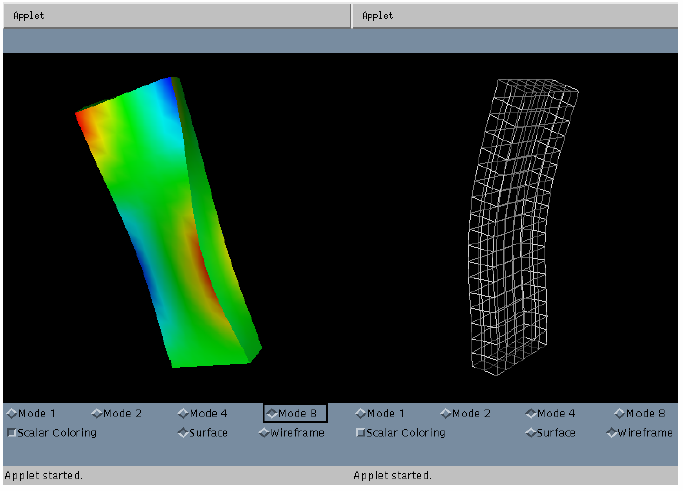
\includegraphics[width=0.8\textwidth]{Figure11-4}\\
  \caption{Two images from a Java (JNI) applet.}\label{fig:Figure11-4}
\end{figure}


The resulting applet is shown in Figure \ref{fig:Figure11-4}.

This demonstrates one of the advantages of using Java for Web visualization. VRML would require that the geometry of each vibrational mode be sent to the client for viewing. With Java and VTK the geometry can be sent once along with a set of scalar displacements for each vibrational mode. Then as the client switches between modes, the geometry can be modified quickly by the client without any additional network traffic. In fact the client could mix vibrational modes or perform an animation showing the vibration of the plate all without having to go back to the server, and without requiring much more data than a single VRML model of the plate. If the client decided to examine another geometry, say the vibrational modes of a disc, then it would likely return to the server for the new data. This is the flexibility that Java provides.
\index{Java|)}\index{visualization!using Java|)}\index{VTK!and Java|)}

\section{Java3D}
\index{Java3D|(}\index{visualization!using Java3D|(}

Similar to a native code implementation (such as a VTK implementation) Java3D provides access to hardware accelerated 3D graphics. Java3D provides both scene graph rendering similar to VRML, and high-level immediate mode rendering. The immediate mode rendering support is not as complete as libraries like OpenGL or DirectX, but it does provide a good subset of its functionality. Java3D does share some of the limitations of native code implementations in that the client must have a version of Java3D for their operating system installed for it to work. There are also some limitations in how both Java3D and native interfaces interact with lightweight GUI components such as swing.

To better understand the Java3D API, we’ll walk through an example applet distributed with the original 1.0 specification. In this example, a colored cube is rendered as it rotates at a fixed rate.

First, let's consider the definition of the cube. Some of the details have been left out for brevity. The complete description of the cube is stored in a Java class we’ll call ColorCube. It contains two class variables (verts and colors) that store the vertex positions and RGB colors. It has an instance of the Shape3D class that will be used by Java3D and a method, getShape(), to access it.

Finally, ColorCube has a constructor that creates a QuadArray, inserts the verts and colors into it, and assigns it to the Shape3D instance variable.

\begin{lstlisting}[language=Java, caption={}, numbers=none, frame=none]
public class ColorCube extends Object
  {
  private static final float[] verts =
    {
    // front face
    1.0f, -1.0f, 1.0f, 1.0f, 1.0f, 1.0f,
    -1.0f, 1.0f, 1.0f, -1.0f, -1.0f, 1.
...
    // bottom face
    -1.0f, -1.0f, 1.0f, -1.0f, -1.0f, -1.0f,
    1.0f, -1.0f, -1.0f, 1.0f, -1.0f, 1.0f,
    };
  private static final float[] colors =
    { // front face (red)
    1.0f, 0.0f, 0.0f, 1.0f, 0.0f, 0.0f,
    1.0f, 0.0f, 0.0f, 1.0f, 0.0f, 0.0f,
...
    // bottom face (cyan)
    0.0f, 1.0f, 1.0f, 0.0f, 1.0f, 1.0f,
    0.0f, 1.0f, 1.0f, 0.0f, 1.0f, 1.0f,
    };
    private Shape3D shape;
    public ColorCube() {
      QuadArray cube = new QuadArray(24,
                          QuadArray.COORDINATES | QuadArray.COLOR_3);
      cube.setCoordinates(0, verts);
      cube.setColors(0, colors);
      shape = new Shape3D(cube, new Appearance());
      }
    public Shape3D getShape() {
      return shape;
      }
  }
\end{lstlisting}

Having defined the geometry, the entry point for a Java3D application is the applet. The HelloUniverse class extends the Applet class and provides the initialization code for this application. The constructor for this applet creates a Canvas3D object that is where the 3D information will be rendered. It then calls the createSceneGraph() method that performs the detailed setup of the scene graph including creating an instance of ColorCube. Then the constructor creates an instance of a UniverseBuilder given the Canvas3D and attaches the scene graph to the Universe. The UniverseBuilder is mostly boiler--plate code that handles setting up the view location (or platform) and attaching it to the Canvas3D.

\begin{lstlisting}[language=Java, caption={}, numbers=none, frame=none]
public class HelloUniverse extends Applet
  {
  public HelloUniverse()
    {
    setLayout(new BorderLayout());
    Canvas3D c = new Canvas3D(graphicsConfig);
    add("Center", c);
    // Create a simple scene and attach it to the virtual universe
    BranchGroup scene = createSceneGraph();
    UniverseBuilder u = new UniverseBuilder(c);
    u.addBranchGraph(scene);
    }
}
\end{lstlisting}

It is worth noting that in the createSceneGraph() method, the use of the previously defined ColorCube class and its insertion into the scene graph via the BranchGroup class. The setCapability() method is used to enable the cube's transform to be modified and underlies an important concept. To achieve the highest rendering rate, Java3D performs a number of optimizations on the scene graph. Many of these optimizations only work if certain properties of the nodes are guaranteed to not change. So by default most properties of a node are set to be ``read only''. To modify them after creation requires the specific call shown below.

\begin{lstlisting}[language=Java, caption={}, numbers=none, frame=none]
public BranchGroup createSceneGraph()
  {
  // Create the root of the branch graph
  BranchGroup objRoot = new BranchGroup();
  // Create the transform group node and initialize it to the
  // identity. Enable the TRANSFORM_WRITE capability so that
  // our behavior code can
  // root of the subgraph.
  TransformGroup objTran = new TransformGroup;
  objTran.setCapability(TransformGroup.ALLOW_TRANSFORM_WRITE);
   objRoot.addChild(objTran);
  // Create a simple shape leaf node, add it to the scene graph.
  objTran.addChild(new ColorCube().getShape());
  // Create a new Behavior object that will perform the desired
  // operation on the specified transform object and add it into
  // the scene graph.
  Transform3D yAxis = new Transform3D;
  Alpha rotationAlpha = new Alpha (
    -1, Alpha.INCREASING_ENABLE, 0, 0, 4000, 0, 0, 0, 0, 0);
  RotationInterpolator rotator =
  new RotationInterpolator(rotationAlpha, objTran, yAxis,
      0.0f, (float) Math.PI*2.0f);
  BoundingSphere bounds =
    new BoundingSphere(new Point3d(0.0,0.0,0.0), 100.0);
  rotator.setSchedulingBounds(bounds); objTran.addChild(rotator);
  objTran.addChild(rotator);
  return objRoot;
}

public void addBranchGraph(BranchGroup bg) {
  locale.addBranchGraph(bg);
   }
\end{lstlisting}
\index{Java3D|)}\index{visualization!using Java3D|)}

\section{VRML, Java, and the EAI}
\index{External Authoring Interface|(}\index{EAI|see {External Authoring Interface}}

The External Authoring Interface (EAI) provides VRML with the same combination of power and flexibility that Java3D has. The EAI provides a communication interface that allows Java and VRML to interact with each other. This is particularly powerful in that a Java applet can create a VRML world, add and delete nodes from the scene graph, and a VRML scene graph can invoke Java code or Java Script in response to an event. In many ways this is similar to the Java3D solution with the exception that VRML is being used for the rendering instead of the Java3D rendering engine. Both solutions have the benefit of Java as a general purpose language for handling programmatic and user-interface issues.

There are a number of ways to organize a visualization that uses the EAI. We will consider the most general method that starts with an HTML page that loads both a VRML world file and a Java applet in the traditional way. This example is loosely derived from work by David Brown. The Java applet starts by importing a number of classes including some VRML specific ones and then defining the instance variables that it will be using.

\begin{lstlisting}[language=Java, caption={}, numbers=none, frame=none]
import java.awt.*;
import java.applet.*;
import java.lang.*;
import vrml.external.field.*;
import vrml.external.Node;
import vrml.external.Browser;
import vrml.external.exception.*;

public class visApplet extends Applet
    {
    // The Browser
    Browser browser = null;
    // Various UI widgets
    Button grow_button, shrink_button;

    // Various stuff in the VRML scene we hang on to
    Node root_node, sphere_node;
    EventInSFVec3f setScale = null;
    float currentScale = (float)1.0;
\end{lstlisting}

Next, the applet defines the init() method that will request a reference to the browser, invoke initScene() to build the VRML interface, and create the user interface. In this case the user interface is just two buttons on a white background.

\begin{lstlisting}[language=Java, caption={}, numbers=none, frame=none]
/** Initialize the Applet */
public void init()
  {
  // Connect to the browser
  browser = Browser.getBrowser(this);
  if (browser == null) {
    die("init: NULL browser!");
  }
  System.out.println("Got the browser: "+browser);

  // Initialize some VRML stuff
  initScene();

  // Build a simple UI
  grow_button = new Button("Grow Sphere");
   add(grow_button);
  shrink_button = new Button("Shrink Sphere");
   add(shrink_button);
  // Misc other UI setup
  Color c = Color.white;
  System.out.println("Setting bg color to: " + c);
   setBackground(c);
}
\end{lstlisting}

There is a simple error handling routine defined.

\begin{lstlisting}[language=Java, caption={}, numbers=none, frame=none]
/** Handle a fatal error condition */
public void die(String s)
   {
   System.out.println("visApplet: FATAL ERROR!");
   System.out.println("--> " + s);
   System.out.println("visApplet: Aborting...\n");
}
\end{lstlisting}

The initScene() method sets up the VRML scene and relies heavily on the EAI. For synchronization reasons, this method starts off by waiting a few seconds to assure that the VRML browser has time to initialize and read the VRML file specified by the HTML. Then it uses the browser.getNode("aName") method to obtain nodes from the scene graph. These nodes must be named using the DEF keyword in the VRML file. The first node it gets is the SPHERE node that happens to be a VRML transform. It uses the getEventIn() method to obtain a handle to the scale instance variable of this transform which will be used later.

\begin{lstlisting}[language=Java, caption={}, numbers=none, frame=none]
/** Set up some stuff in the VRML scene */
    public void initScene()
      {
      System.out.println("initScene()...");

     // wait a couple seconds
     try {
       Thread.currentThread().sleep(5000);
       }
     catch(InterruptedException e) {}
     // Get the "SPHERE" node
      try {
       sphere_node = browser.getNode("SPHERE");
       }
      catch(InvalidNodeException e) {
        System.out.println("InvalidNodeException: " + e);
        die("initScene: SPHERE node not found!");
        return;
        }
      System.out.println("- Got the SPHERE node: " + sphere_node);
      try {
        setScale = (EventInSFVec3f)
        sphere_node.getEventIn("set_scale");
        }
      catch (InvalidEventInException e) {
        die("initScene: InvalidEventInException " + e);
        return;
        }
\end{lstlisting}

Then the same techniques are used to obtain the ROOT node of the scene graph. If you scan the VRML file that follows this example, you will see that the ROOT node is just an empty Group. After obtaining the node we request handles to its addChildren() and removeChildren() methods.

\begin{lstlisting}[language=Java, caption={}, numbers=none, frame=none]
    // Get the "ROOT" node (a Group which we add to)
    try {
      root_node = browser.getNode("ROOT");
      }
    catch(InvalidNodeException e) {
      System.out.println("InvalidNodeException: " + e);
      die("initScene: ROOT node not found!");
    return;
    }
  System.out.println("- Got the ROOT node: " + root_node);

  // Get the ROOT node's add/removeChildren
  EventIns EventInMFNode addChildren;
  EventInMFNode removeChildren;
  try {
    addChildren = (EventInMFNode)
    root_node.getEventIn("addChildren");
    removeChildren = (EventInMFNode)
    root_node.getEventIn("removeChildren");
    }
  catch (InvalidEventInException e) {
    die("initScene: InvalidEventInException " + e);
    return;
    }
\end{lstlisting}

Using the EAI, VRML can be created from a Java string as shown in the following code. This allows us to create geometry on the fly and add it to the scene graph using the addChildren() handle obtained above. The handles support matching setValue() and getValue() methods that modify and interrogate the scene graph respectively.

\begin{lstlisting}[language=Java, caption={}, numbers=none, frame=none]
// Create the VRML for a purple sphere
Node[] shape;
String purple_sphere =
  "#VRML V2.0 utf8\n" +
  "Transform {\n" +
  "  children Shape {\n" +
  "     appearance Appearance {\n" +
  "       material Material {\n" +
  "         diffuseColor 0.8 0.2 0.8\n" +
  "     }\n" +
  "   }\n" +
  "   geometry Sphere {}\n" +
  " }\n
  " translation 0 3 0" +
  "}\n";
  try {
    shape = browser.createVrmlFromString(purple_sphere);
    }
  catch (InvalidVrmlException e) {
    die("initScene: InvalidVrmlException: " + e);
    return;
    }
  // Add the sphere to the ROOT group
  addChildren.setValue(shape);
  System.out.println("initScene: done.");
  }
\end{lstlisting}

The events for the two buttons are processed in the action() method. One increases the scale of the sphere and the other decreases it. This is done using the handle to the SPHERE node's scale that was obtained in the initScene() method, and invoking the setValue() method with the appropriate arguments.

\begin{lstlisting}[language=Java, caption={}, numbers=none, frame=none]
/** Handle actions from AWT widgets */
    public boolean action(Event event, Object what)
      {
      if (event.target instanceof Button) {
      Button b = (Button) event.target;
      if (b == grow_button) {
        currentScale = currentScale * (float)1.2;
        float ascale[] = new float[3];
        ascale[0] = currentScale;
        ascale[1] = currentScale;
        ascale[2] = currentScale;
        setScale.setValue(ascale);
        }
      else if (b == shrink_button) {
        currentScale = currentScale / (float)1.2;
        float ascale[] = new float[3];
        ascale[0] = currentScale;
        ascale[1] = currentScale;
        ascale[2] = currentScale;
        setScale.setValue(ascale);
        }
      } // event.target instanceof Button
      return true;
\end{lstlisting}

The events for the two buttons are processed in the action() method. One increases the scale of the sphere and the other decreases it. This is done using the handle to the SPHERE node's scale that was obtained in the initScene() method, and invoking the setValue() method with the appropriate arguments.

\begin{lstlisting}[language=Java, caption={}, numbers=none, frame=none]
/** Handle actions from AWT widgets */
    public boolean action(Event event, Object what)
      {
      if (event.target instanceof Button) {
      Button b = (Button) event.target;
      if (b == grow_button) {
        currentScale = currentScale * (float)1.2;
        float ascale[] = new float[3];
        ascale[0] = currentScale;
        ascale[1] = currentScale;
        ascale[2] = currentScale;
        setScale.setValue(ascale);
        }
      else if (b == shrink_button) {
        currentScale = currentScale / (float)1.2;
        float ascale[] = new float[3];
        ascale[0] = currentScale;
        ascale[1] = currentScale;
        ascale[2] = currentScale;
        setScale.setValue(ascale);
        }
      } // event.target instanceof Button
      return true;
}
\end{lstlisting}

The last method in the applet draws a border around the two buttons when the applet needs to be repainted.

\begin{lstlisting}[language=Java, caption={}, numbers=none, frame=none]
/** Override paint() to get more control over how we're drawn */
 public void paint(Graphics g)
   {
   int w = size().width;
   int h = size().height;

   // Draw a simple border
   g.drawRect(0, 0, w-1, h-1);
   g.drawRect(1, 1, w-3, h-3);
   super.paint(g);
   }
}
\end{lstlisting}

\begin{figure}[!htb]
  \centering
  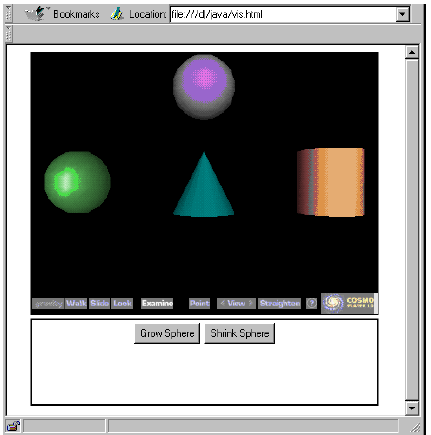
\includegraphics[width=0.8\textwidth]{Figure11-5}\\
  \caption{ Java and VRML combined using the EAI.}\label{fig:Figure11-5}
\end{figure}

An excerpt from the VRML file has been included below. Note the use of the DEF keyword to name nodes that can then be accessed from Java. The resulting Java/VRML example can be seen in Figure \ref{fig:Figure11-5}.

\begin{lstlisting}[language=VRML, caption={}, numbers=none, frame=none]
#VRML V2.0 utf8
#
Group {
  children [ 
    #
    # Some objects
    #
    DEF ROOT Group {}
    DEF SPHERE Transform {
      childrenShape {
        appearanceAppearance {
          materialMaterial {
            ambientIntensity 0.283774
            diffuseColor 0.0846193 0.56383 0.0595097
            specularColor 0.13092 0.87234 0.0920716
            emissiveColor 0 0 0
            shininess 0.2
            transparency 0
          }
       }
       geometrySphere {}
     }
     translation-4 0 0
   }
  ]
}
\end{lstlisting}
\index{External Authoring Interface|)}

\section{The Future of Web Visualization}

In the previous sections we provided an overview of some of the technologies important to applying visualization on the World Wide Web. Since Web-based technologies, computer graphics, and visualization are all rapidly growing fields, the likelihood of new development and change is high. However, we are confident that these technologies will remain important to the future. Eventually we expect 3D graphics and data visualization to become as pervasive as 2D graphical user interfaces and presentations are today. The main barriers to this development is the limited bandwidth of the Web, lack of familiarity (and difficulty of use) of 3D graphics and visualization, and limitations in computer hardware and software. We believe that technological advances will eventually minimize bandwidth and computer hardware limitations, while systems like VTK will make 3D graphics and visualizations easier to use.

One of the benefits of systems like VTK is that they are driven by their algorithmic content. The systems we have seen earlier such as OpenGL, HTML, VRML and Java, are implementations of a system or information protocol. Algorithmic systems, on the other hand, implement mathematical, logical, and design relationships that change much more slowly than system implementations. As a result, systems like VTK will remain vital for years to come, although the underlying implementation language and interface may change. To track future changes to VTK visit our Web pages at \href{https://www.vtk.org/}{https://www.vtk.org/}.

\section{Chapter Summary}

Visualization over the Web opens up many forms of collaborative development, entertainment, and publishing that were previously restricted to a few individuals with access to custom software. There are many ways to perform visualization over the Web ranging from simple HTML pages with pictures, to complete Java-based applications. Deciding on the correct solution for Web visualization depends on three key factors: 1) the amount of interaction and control you want to provide to the user or client, 2) performance issues related to data size and client/server load balancing, 3) how much complexity you are willing to deal with. While the Java-based solutions can provide interaction, control, and load balancing, this involves added complexity. It may be that producing a static VRML file for your Web page is sufficient. Either way there are a host of tools available and more are on the way. The greatest challenge will likely be to create a future standard for the Web that includes not just 3D viewing but also visualization.

\section{Bibliographic Notes}
\label{sec:ch11.bibliographic_notes}

For a general introduction to HTML and CGI consider \cite{Morris95} or \cite{Graham95}. Both books provide a good introduction and include coverage for both UNIX and MS Windows-based systems. For more detailed coverage of CGI programming consider \cite{Gundavaram96}. Mark Pesce \cite{Pesce95} provides a n excellent introduction to VRML including its early genesis. \cite{Ames96} is also a great VRML resource. The Inventor Mentor by Josie Wernecke \cite{Wernecke94} is an excellent book for learning about Open Inventor and scene graphs. Java in a Nutshell \cite{Flanagan96} is a good reference for Java and for someone who already knows how to program in another language For documentation on the Java Native Interface or Java3D, visit Sun's Web site at \href{https://www.java.com/en/}{Java}.


\printbibliography
